\documentclass[12pt, a4paper]{article}
\usepackage[letterpaper, portrait, margin=1 in]{geometry}
\usepackage{amsmath}
\usepackage{amsfonts}
\usepackage{xcolor}
\usepackage{cite}
\usepackage{amssymb}
\usepackage{setspace}
\newcommand*\diff{\mathop{}\!\mathrm{d}}
\newcommand*\Diff[1]{\mathop{}\!\mathrm{d^#1}}
\usepackage{graphicx} 

\begin{document}
\doublespacing

\section{Background} 

$\indent$ Survival and reproduction are key elements of a successful population. Lifetimes can provide information about population growth and size, and recruitment times can inform population growth rates. Recruitment times are defined as the time it takes for an individual to become parous, or to reproduce for the first time. Both survival rates and  recruitment may be affected by environmental factors and can influence the health and stability of a population. We investigated the lifetime and recruitment time in a population of California sea lions. Estimates of these population parameters can be used by researchers to assess population trends over time for management, conservation, and scientific purposes.  

The data are from a long-term capture-resight study conducted by Melin et al on San Miguel Island \cite{Melin}. Between 1987 and 2001, researchers branded 3945 healthy 4-5 month old female sea lion pups. The researchers took observations of the population during the summers in the years 1991-2008, recording each time a branded sea lion was resighted. They recorded the sea lion's brand number, date and location of resight, and indicated if the sea lion was seen with her own pup or not. This long-term capture-resight study provides useful data for estimating various population parameters, specifically time until recruitment and death. 

\section{Build Model}

We analyzed a subset of the data consisting of a cohort of 259 female sea lion pups branded in 1991 and resighted between 1992 and 2008. To estimate time until recruitment, $r_i$, and time until death, $d_i$, for each individual in the 1991 cohort, we fit the following hierarchical model. \\
\\
For $i = 1, \ldots n$, $t = 1, \ldots, T$, and $r_i \leq d_i$ for all $i$, 

\begin{eqnarray*}
y_{it} & \sim & \begin{cases} 0 & , t \leq r_i \\
\text{Bern}(p) & , t > r_i \end{cases} \\
z_{it} & \sim & \begin{cases} 0 & , t > d_i \\
\text{Bern}(\psi) & , t \leq d_i \end{cases} \\
f &=& (.8)*\frac{1}{8} \exp(-\frac{x}{8}) + (.2)*\frac{1}{3\sqrt{2\pi}} \exp \left(-\frac{1}{18} (x - 25)^2 \right) \\
d_i & \propto & f * 1_{(d_i > t_i^*)} \\
\log(r_i) & \sim & \text{N}(\mu_r, \sigma_r^2) \\
\mu_r & \sim & \text{N}(\mu_0, \sigma_0^2) \\
\sigma_r^2 & \sim & \text{IG}(\alpha_{\sigma}, \beta_{\sigma}) \\
p & \sim & \text{Beta}(\alpha_p, \beta_p) \\
\psi & \sim & \text{Beta}(\alpha_{\psi}, \beta_{\psi} )\\
\end{eqnarray*}
where $y_{it}$ indicates if individual $i$ was observed with a pup in year $t$, $z_{it}$ indicates if individual $i$ was observed in year $t$. The parameter $d_i$ denotes time until individual $i$ left the population. This could be due to either death or emigration. The constant $t_i^*$ denotes the last time individual $i$ was observed in the study. The parameter $r_i$ denotes the time until individual $i$ became parous.
The probability of an individual being detected with her pup assuming she was alive, at the site, and parous is denoted $p$. Therefore, $p$ includes both the probability that a parous female had a pup and that she was observed alongside her pup. The probability of detecting an individual given that she was alive and at the site is given by $\psi$. 

\section{Prior Specification}

The prior distribution for $d_i$ is proportional to an 80/20 mixture of an exponential distribution with mean 8 and a normal distribution with mean 25 and variance 9. According to previous research studying age-specific survival rates of California sea lions \cite{Hernandez}, the probability of a young female sea lion surviving the first year of life ranges from .558 to .998. After the first year, the probability of survival from year $t$ to year $t+1$ is roughly 0.9 \cite{Hernandez}. Our prior specification for $d_i$ emulates this prior knowledge. The prior probability of survival to year 1 is 0.705, to year 4 is .485, and to year 10 is .43. This reflects lower survival probabilities for young and old individuals and higher survival probabilities for middle-aged individuals. We include in our prior distribution on $d_i$ the fact that if an individual $i$ was last seen at time $t_i^*$, then $d_i$ must be greater than $t_i^*$. 

We chose the prior hyperparameters for $\mu_r$ and $\sigma_r^2$ based off recent research on South American sea lions. In a study by Grandi et al, researchers estimated that female South American sea lions reach sexual maturity around 4.8 $\pm$ 0.5 years \cite{Grandi}. We believed California sea lions would mature at a similar age and therefore let $\mu_0 = 1.6$ and $\sigma_0^2 = .0625$, roughly corresponding to an average recruitment time of 5 years and allowing for moderate variation around this mean. We let $\alpha_{\sigma} = 3$ and $\beta_{\sigma} = 1$ so the expected variation in $\log(r_i)$ is E$[\sigma_r^2] = 0.5$ and Var$[\sigma_r^2] = 0.25$. This allows individual recruitment times to have reasonable variability around the mean. 

We set the prior hyperparameters for $p$ as $\alpha_p = 1.5$ and $\beta_p = 4.5$. Then E$[p] = .25$, with a fair amount of uncertainty around this mean. This reflects the idea that we do not have a great deal of information regarding $p$, but we believe $p$ may be relatively low since not all fertile sea lions reproduce and mothers may be spotted without their pups. We set the hyperparameters for $\psi$ as $\alpha_{\psi} = 2$ and $\beta_{\psi} = 2$. This corresponds to E$[\psi] = .5$, with most mass centered around .5 and much less mass near 0 and 1. This reflects the idea that we believe $\psi$ is likely to be higher than $p$, but we still have little information regarding this parameter.  

\section{Posterior Distribution}
\begin{eqnarray*}
[\log (\mathbf{r}), \mu_r, p, \mathbf{d}, \lambda, \psi | \mathbf{z}, \mathbf{y} ] & \propto & \prod_{i=1}^n \prod_{t=1} ^T  1\{r_i \leq d_i \} [y_{it}|p,r_i]^{1\{ t > r_i \}} 1^{1\{ t \leq r_i \}} [z_{it}|\psi, d_i]^{1 \{ t \leq d_i\} } 1^{1 \{ t > d_i\}} \\
  & \times & [\log(r_i)|\mu_r][d_i|\lambda]  [\mu_r][\lambda][p][\psi]
\end{eqnarray*}


\section{Algorithm}

We derived the full conditionals for $p$, $\psi$, $\mu_r$, and $\sigma_r^2$ (Appendix) and updated those parameters with a Gibbs sampler. We updated $\mathbf{d}, \mathbf{r}$, and with Metropolis-Hastings. We ran the MCMC algorithm for 100,000 iterations with a burn-in period of 50,000. Resulting trace plots showed thorough mixing and convergence of parameters . 

\section{Results}

\begin{table}[ht]
\centering
\begin{tabular}{rrrr}
  \hline
   & Posterior Mean & 95\% CI Lower & 95\% CI Upper \\ 
  \hline
  p & 0.12 & 0.10 & 0.13 \\ 
  psi & 0.27 & 0.25 & 0.30 \\ 
   \hline
\end{tabular}
\end{table}

\begin{figure}
\centering
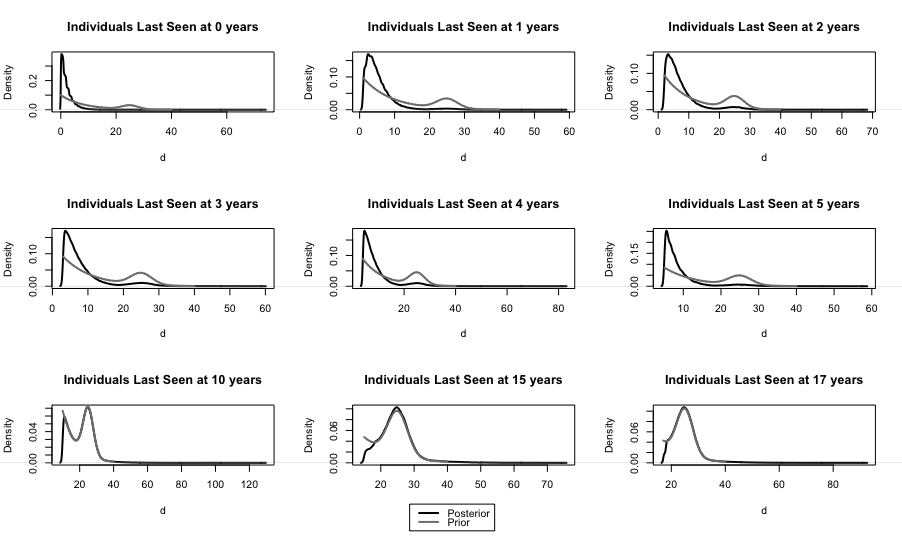
\includegraphics[width = \textwidth]{Posterior.d.png}
\caption{Posterior distribution on $d$ for individuals which we last saw in certain years.}
\end{figure}

\section{Inference}

Ideally, the parameter $d_i$ represents the lifetime of individual $i$, but practically it represents the time the individual left the population, which could be due to death or emigration. Future research could address this issue by also modeling the probability of emigration using some sort of spatial tracking mechanism. 

Our model predicts varying times for $d_i$ based on the last time the individual $i$ was observed in the study period. For individuals not observed after the first few years, the estimated time in the population tended to relatively low, with most mass below 10 years. For individuals observed later into the study, the estimated time in the system tended to be dominated by the prior distribution, and the posterior mass was concentrated around 25 years. If an individual was only observed in the first few years of the study, it may be due to the fact that it was simply never detected, but our posterior distribution reflects substantial probability that the individual actually left the system. Due to strong prior information that the expected life time for California sea lions is around 20-30 years, individuals that were observed late into the study period had a high posterior probability of remaining in the system for 20-30 years. 

The parameter $\psi$ denotes the probability of detecting an individual assuming she was alive and at the site. Our posterior mean for $\psi$ is $0.27 (95\% CI: [.25, .30])$. 

The parameter $p$ is a complex parameter in this model. It assumes an individual is alive, parous, and at the site and includes the probability of a parous female having a pup and of the researchers observing her with her pup. The posterior mean for $p$ is $0.12 (95\% CI: [.10, 13])$. This relatively low detection probability is not surprising given there are many reasons that an individual with a pup may not be detected with her pup. Not long after birth, sea lion mothers tend to leave their pups to hunt, so it is possible to detect a sea lion without her pup even if she had a pup in that year. Furthermore, not all parous females have pups ever year, and this probability is included in $p$. 

The data from this research study also included repeated sightings within a year. This model could be improved upon by utilizing the within-year sightings to inform the detection probabilities $p$ and $\psi$. 

Our posterior distributions for $r_i$, the time until individual $i$ became parous, were not substantially different across individuals that were last sighted at different times.  The posterior means for $r_i$ were typically between 0.243 and 2.004 years. Based on prior information that sea lions typically become parous around 4-5 years, our model is under-estimating this parameter. This is likely due to the low probability of detecting an individual with her pup and the constraint that $r_i < d_i$. This constraint might be relaxed in the future, since an individual may in fact die or leave the population before she ever becomes parous. In this case we would have $d_i < r_i$, where $r_i$ is the theoretical time at which the individual would have become parous if she had lived or remained in the population long enough. 




\section{Appendix}

% \subsection{Full Conditionals} 
% 
% Full conditional distributions were derived for the parameters $p$, $\psi$, $\lambda$, and $\sigma_r^2$:
% \begin{eqnarray*}
% p | \cdot & \sim & \text{Beta} \left( \alpha_p + \sum_{i=1}^n \sum_{t=1}^T 1 \{ r_i \leq t \leq d_i \} y_{it}, \beta_p + \sum_{i=1}^n \sum_{t=1}^T 1\{ r_i \leq t \leq d_i \} (1 - y_{it}) \right)  \\
% \psi | \cdot & \sim & \text{Beta}\left( \alpha_{\psi} + \sum_{i=1}^n \sum_{t=1}^T 1\{ t \leq d_i\} z_{it}, \beta_{\psi} + \sum_{i=1}^n \sum_{t=1}^T 1\{ t \leq d_i \} (1 - z_{it}) \right) \\
% \sigma_{r}^2 | \cdot & \sim & \text{IG} \left( \alpha_{\sigma} + \frac{n}{2}, \beta_{\sigma} + \frac{1}{2} \sum_{i=1}^n ( \log(r_i) - \mu_r)^2 \right)
% \end{eqnarray*}
% The parameters $\mathbf{d}, \mathbf{r}$, and $\mu_r$, did not have recognizable full conditionals so we updated them with Metropolis-Hastings.  

\begin{thebibliography}{99}

\bibitem{NOAA}
NOAA: California Sea Lion, \\
\text{http://www.nmfs.noaa.gov/pr/species/mammals/sealions/california-sea-lion.html}

\bibitem{Grandi}
Grandi, M.F., Dans, S.L., Garcia, N.A., Crespo, E.A. 2010. \emph{Growth and age at sexual maturity of South American sea lions}. Mammalian Biology, 75(5):427-436.   

\bibitem{Melin}
Melin, Sharon R.; DeLong,Robert L.; Orr, Anthony J.; Laake, Jeffrey L.; Harris, Jeffrey D.; NOAA NMFS Alaska Fisheries Science Center, Marine Mammal Laboratory (2016). Survival and natality rate observations of California sea lions at San Miguel Island, California conducted by Alaska Fisheries Science Center, National Marine Mammal Laboratory from 1987-09-20 to 2014-09-25 (NCEI Accession 0145167). Version 2.2. NOAA National Centers for Environmental Information. Dataset. [Nov. 19, 2017]

\bibitem{Hernandez}
Hernandez-Camacho, Claudia J.; Aurioles-Gamboa, David; Laake, Jeffrey; Gerber, Leah R. 2008. Survival Rates of the California Sea Lion, Zalophus californianus, in Mexico, Journal of Mammalogy, 89(4): 1059–1066, https://doi.org/10.1644/07-MAMM-A-404.1


\end{thebibliography}

\end{document}
